\documentclass{article}

\usepackage{graphicx}
\usepackage{tikz}
\usepackage{tikzsymbols}
\usetikzlibrary{calc,patterns,shapes.geometric}
\pagestyle{empty}
\usepackage[margin=0pt]{geometry}
\geometry{papersize={14in,12in}}

\def\centerarc[#1](#2)(#3:#4:#5){\draw[#1] ($(#2)+({#5*cos(#3)},{#5*sin(#3)})$) arc (#3:#4:#5);}

\begin{document}
	\begin{figure}
		\centering
		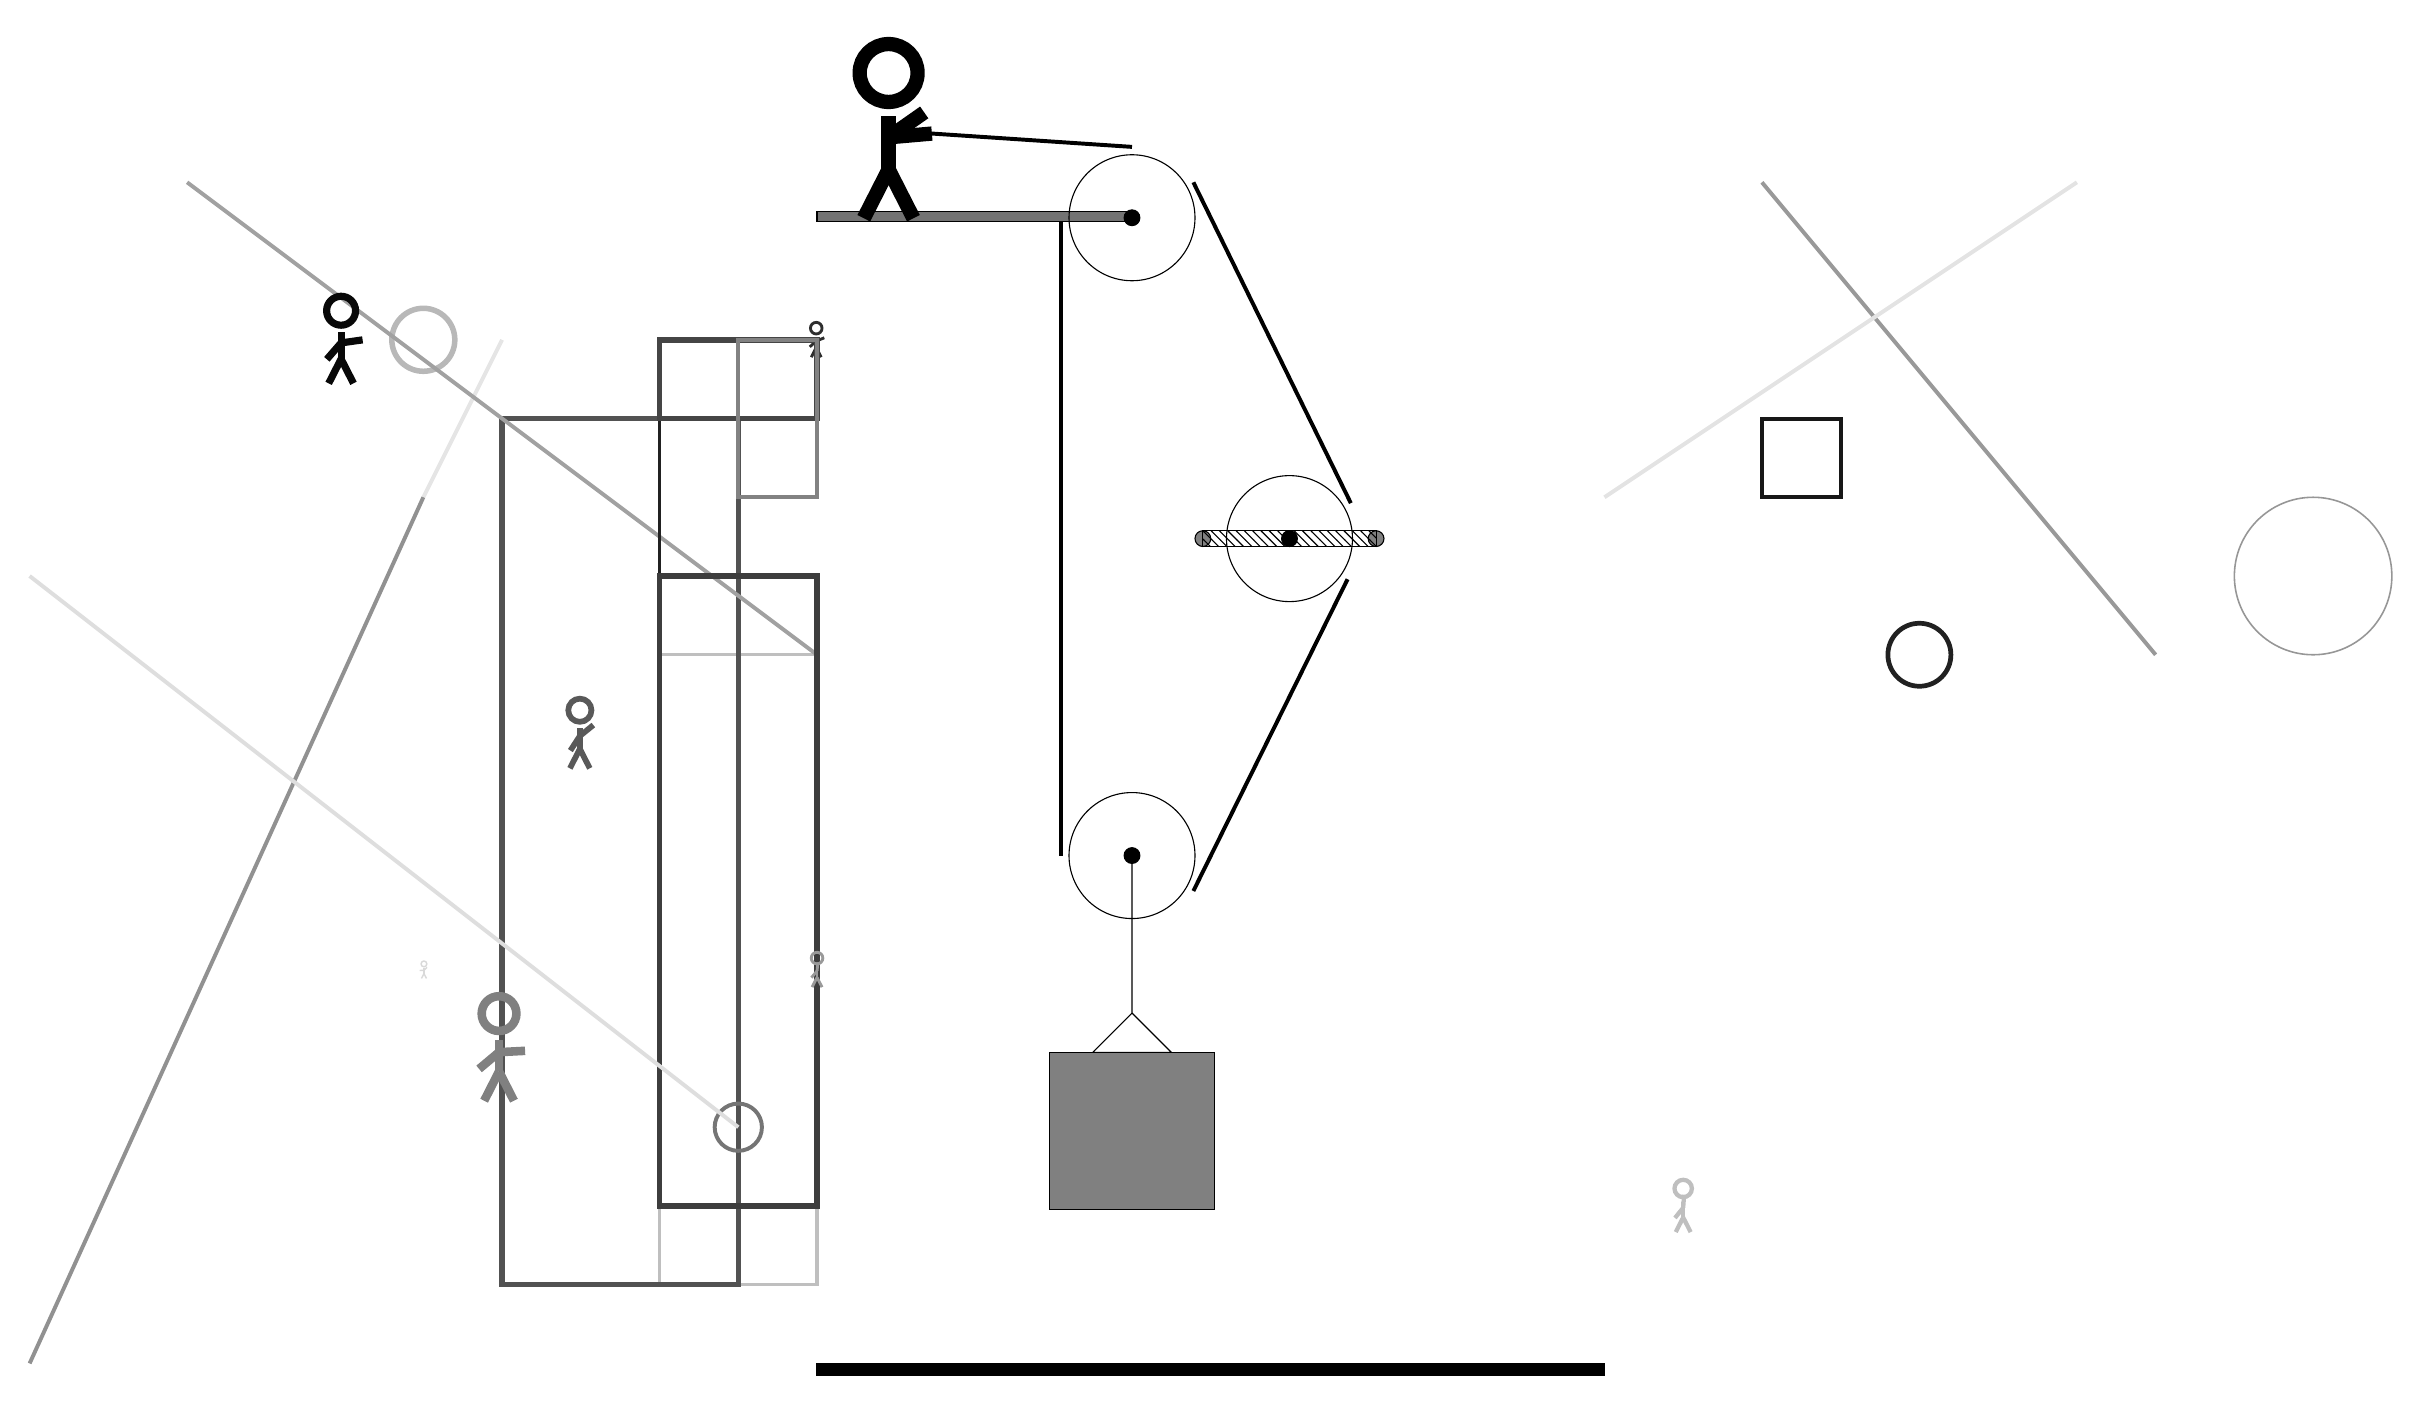
\begin{tikzpicture}
			%%%%% START %%%%%
			
			\draw[fill=black!55] (-2, 11.5) rectangle (2, 11.625);
			
			\draw (2, 3.45) circle (0.8);
			\draw[fill=black] (2, 3.45) circle (0.1);
			
			\draw (2, 11.55) circle (0.8);
			\draw[fill=black] (2, 11.55) circle (0.1);
			
			\draw[fill=white](4, 7.475) circle (0.8);
			\draw[fill=black] (4, 7.475) circle (0.1);
			\draw[fill=black!50] (2.9, 7.475) circle (0.1);
			\draw[fill=black!50] (5.1, 7.475) circle (0.1);
			\draw[pattern=north west lines, pattern color=black] (2.9, 7.575) rectangle (5.1, 7.375);
			
			\draw (2, 3.45) -- (2, 1.45) -- (1.5, 0.95) -- (2.5, 0.95) -- (2, 1.45);
			\draw[fill=black!50] (0.95, 0.95) rectangle (3.05, -1.05);
			
			\draw[line width=0.5mm] (1.1, 11.5) -- (1.1, 3.45);
			\centerarc[line width=0.5mm](2, 3.45)(180:330:0.9);
			\draw[line width=0.5mm](2.7794, 3.0) -- (4.7373, 6.9588);
			\centerarc[line width=0.5mm](4, 7.475)(390:325:0.9);
			\draw[line width=0.5mm](4.7794, 7.925) -- (2.7794, 12.0);
			\centerarc[line width=0.5mm](2, 11.55)(30:90:0.9);
			\draw[line width=0.5mm](2, 12.45) -- (-1, 12.65);
			
			\draw[line width=0.5mm, color=black!10](-6, 10) -- (-7, 8);
			
			\draw[line width=0.5mm, color=black!40](10, 12) -- (15, 6);
			\node[line width=0.5mm, color=black!82] at (-2, 10) {\Strichmaxerl[2][42][22]};
			\draw[line width=0.5mm, color=black!43](-7, 8) -- (-12, -3);
			\draw[line width=0.4mm, color=black!25] (-4, 6) rectangle (-2, -2);
			\node[line width=0.7mm, color=black!65] at (-5, 5) {\Strichmaxerl[4][57][39]};
			
			\draw[line width=0.5mm, color=black!11](8, 8) -- (14, 12);
			\draw[line width=0.7mm, color=black!68] (-3, 9) rectangle (-6, -2);
			\draw [line width=0.7mm, color=black!28](-7, 10) circle (0.4);
			
			\draw [line width=0.2mm, color=black!41](17, 7) circle (1.0);
			
			\draw[line width=0.5mm, color=black!37](-2, 6) -- (-10, 12);
			\node[line width=0.5mm, color=black!97] at (-8, 10) {\Strichmaxerl[5][49][8]};
			\draw[line width=0.5mm, color=black!91] (10, 9) rectangle (11, 8);
			\node[line width=0.4mm, color=black!50] at (-6, 1) {\Strichmaxerl[6][40][3]};
			\draw [line width=0.5mm, color=black!54](-3, 0) circle (0.3);
			\draw[line width=0.3mm, color=black!87] (-4, 10) rectangle (-4, 0);
			\draw[line width=0.7mm, color=black!76] (-4, -1) rectangle (-2, 7);
			\node[line width=0.3mm, color=black!40] at (-2, 2) {\Strichmaxerl[2][50][84]};
			\draw[line width=0.7mm, color=black!73] (-2, 9) rectangle (-4, 10);
			\draw[line width=0.5mm, color=black!13](-3, 0) -- (-12, 7);
			\draw [line width=0.6mm, color=black!87](12, 6) circle (0.4);
			
			\draw[line width=0.5mm, color=black!49] (-2, 10) rectangle (-3, 8);
			\node[line width=0.7mm, color=black!25] at (9, -1) {\Strichmaxerl[3][51][86]};
			\node[line width=0.4mm, color=black!15] at (-7, 2) {\Strichmaxerl[1][2][44]};
			
			\node at (-1, 12.65) {\Strichmaxerl[10][-175][35]};
			
			\draw[fill=black] (-2, -3) rectangle (8, -3.15);
			
			%%%%% END %%%%%
		\end{tikzpicture}
	\end{figure}	
\end{document}